\documentclass{article}
\usepackage[T1]{fontenc}
\usepackage{lmodern}
\usepackage{graphicx}
\usepackage{amsmath,amssymb}
\usepackage[a4paper,margin=2cm]{geometry}
\usepackage[absolute,overlay]{textpos}
\setlength{\TPHorizModule}{1mm}
\setlength{\TPVertModule}{1mm}
\usepackage[indonesian]{babel}
\usepackage{hyperref}
\setlength{\emergencystretch}{2em}
% unit: Halaman 64

\begin{document}

% === Halaman 64 (python/native) ===

• Pada setiap putaran, proses enciphering 

melibatkan operasi substitusi dan 

permutasi. Operasi substitusi dilakukan 

dengan cara operasi look-up tabel S

• Operasi substitusi, diikuti dnegan 

oeprasi permutasi dilakukan pada setiap 

putaran. Setiap putaran menggunakan 

kunci putaran yang berbeda-beda (K1, 

K2, K3, dst).

• Operasi substitusi menghasilkan efek 

confusion, sedangkan operasi permutasi 

menghasilkan efek diffusion.

https://commons.wikimedia.org/w/index.php?curid=6420152

64

% deskripsi: gambar native xref 253
\noindent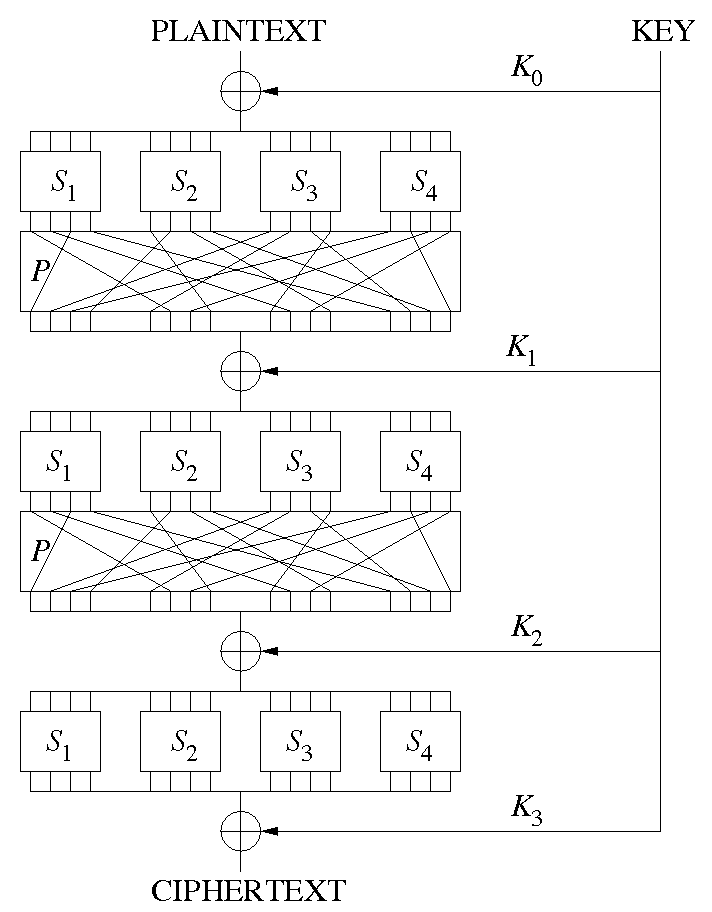
\includegraphics[width=0.85\textwidth]{../../images/python/page_064_img_01.png}

\end{document}
